\subsection{Overlapping Periods}

When plotting the boundaries of the chains of parameter regions with the same period, we see that they overlap.
\Cref{fig:state.og.overlapping.chains} shows the edges of regions of the same period when scanned from different directions.
The scan from left to right is colored in yellow, and from right to left in purple.
At most points, they agree with the corresponding scans from top to bottom in red and from bottom to top in blue, respectively.
When starting in an area of coexistence, blue, purple, yellow, and red show some disagreements.
This is apparent in the zoomed-in \Cref{fig:state.og.overlapping.chains.zoomed}.
The reason is that in these regions of coexistence, \hl{where the chains overlap}, the cycles sometimes start on one cycle and sometimes on \hl{another cycle with a different period}.
\hl{This causes, for example, the yellow lines in the lower left area of \Cref{fig:state.og.overlapping.chains.zoomed}.}
When the scans start in an area, where just one period exists, they agree \hl{most of the time.}
There is another exception, that is the scans from top to bottom in red and from bottom to top in blue can't detect the ``teeth'' because they \hl{don't detect the coexisting cycle right away.}

\begin{figure}
	\centering
	\begin{subfigure}{0.4\textwidth}
		\includegraphics[width=\textwidth]{99_Yunus/2D_Regions_Zoomed/result.png}
		\caption{Overview}
		\label{fig:state.og.overlapping.chains}
	\end{subfigure}
	\begin{subfigure}{0.4\textwidth}
		\includegraphics[width=\textwidth]{99_Yunus/2D_Regions_Zoomed2/result.png}
		\caption{Zoomed In}
		\label{fig:state.og.overlapping.chains.zoomed}
	\end{subfigure}
	\caption[2D scan of the edges of parameter regions with different periods in the original model]{
		2D scan of the edges of parameter regions with different periods in the original model.
		The parameters $\beta = 1, f = 150, L = 4.2 \cdot 10^{-3}, R = 2, V_m = 5,$ and $\mu = 0.5$ are fixed.
		In (a), the parameters $E_0$ and $\chi_0$ are varied in the ranges $[14, 28]$ and $[0.1, 0.65]$, respectively.
		(b) shows a zoomed-in version with the parameters $E_0$ and $\chi_0$ being varied in the ranges $[16.4, 17.2]$ and $[0.16, 0.22]$, respectively.
	}
\end{figure}

\hl{
	A trick allows us to also plot the boundaries of single ``type A'' and ``type B'' parameter regions.
	Adjusting the model to only act on the state space $[0, \pi]$, using the symmetry, the ``type B'' parameter regions now have a much higher period than the ``type A'' parameter regions of the same chain.
	This will be explained in-depth in \Cref{chap:add}, for now it is only important that it allows us to see ``type B'' parameter regions.
}
\Cref{fig:state.og.overlapping.regions.zoomed} shows this for the zoomed-in scan in \Cref{fig:etup.og.overlapping.chains.zoomed} from above.
You can see there that the ``type A'' and ``type B'' parameter regions also overlap.
\hl{
	\Citeauthor{akyuz2022} found in his thesis that in such an overlap of 2 parameter regions there are 3 coexisting stable cycles, one cycle of the ``type A'' parameter region and 2 cycles from the ``type B'' parameter region.
}

\begin{figure}
	\centering
	\includegraphics[width=0.6\textwidth]{98_Yunus_modpi/2D_Regions_Zoomed2/result.png}
	\caption[2D scan of the edges of parameter regions with different periods in the adjusted original model]{
		2D scan of the edges of parameter regions with different periods in the adjusted original model.
		The parameters $\beta = 1, f = 150, L = 4.2 \cdot 10^{-3}, R = 2, V_m = 5,$ and $\mu = 0.5$ are fixed.
		The parameter ranges of $E_0$ and $\chi_0$ are the same as in \Cref{fig:state.og.overlapping.chains.zoomed}, $[16.4, 17.2]$ and $[0.16, 0.22]$, respectively.
		Here, we can see the boundaries of ``type B'' parameter regions as they have higher periods in the adjusted model.
	}
	\label{fig:etup.og.overlapping.regions.zoomed}
\end{figure}
